%ADD INTRO TO CLASSIFICATION
% two target variables → detail binned rating
% knn: only numeric, NB and DT: both numeric and all feats
% detail evaluation → classification report, conf matrix, ROC AUC score (although not relevant bc the dataset is unbalanced), PR curve and AUC
% dummy classifier benchmarks for the two target variables

\begin{table}[h]
    \centering
    \small
    \setlength{\tabcolsep}{4pt}
    \renewcommand{\arraystretch}{0.9}
    \begin{tabular}{lcccc}
        \hline
        & \textbf{precision} & \textbf{recall} & \textbf{f1-score} & \textbf{support} \\
        \hline
        movie & 0.353 & 0.331 & 0.341 & 1877 \\
        short & 0.162 & 0.183 & 0.172 & 766 \\
        tvEpisode & 0.275 & 0.282 & 0.278 & 1599 \\
        tvMiniSeries & 0.027 & 0.025 & 0.026 & 81 \\
        tvMovie & 0.059 & 0.057 & 0.058 & 299 \\
        tvSeries & 0.076 & 0.081 & 0.078 & 447 \\
        tvShort & 0.000 & 0.000 & 0.000 & 16 \\
        tvSpecial & 0.016 & 0.020 & 0.018 & 49 \\
        video & 0.035 & 0.032 & 0.033 & 250 \\
        videoGame & 0.013 & 0.011 & 0.012 & 94 \\
        \hline
        accuracy & & & \textbf{0.233} & 5478 \\
        macro avg & 0.102 & 0.102 & \textbf{0.102} & 5478 \\
        \hline
    \end{tabular}
    \caption{Classification report for the Dummy Classifier on \textit{titleType}.}
    \label{tab:class_report_dummy_titleType}
\end{table}

\begin{table}[h]
    \centering
    \small
    \setlength{\tabcolsep}{3pt}
    \renewcommand{\arraystretch}{0.9}
    \begin{tabular}{p{2.1cm}cccc}
        \hline
        & \textbf{precision} & \textbf{recall} & \textbf{f1-score} & \textbf{support} \\
        \hline
        Low & 0.277 & 0.268 & 0.273 & 1542 \\
        Medium-low & 0.267 & 0.275 & 0.271 & 1522 \\
        Medium-high & 0.305 & 0.312 & 0.309 & 1608 \\
        High & 0.141 & 0.135 & 0.138 & 806 \\
        \hline
        accuracy & & & \textbf{0.264} & 5478 \\
        macro avg & 0.248 & 0.248 & \textbf{0.248} & 5478 \\
        \hline
    \end{tabular}
    \caption{Classification report for the Dummy Classifier on \textit{binned rating}.}
    \label{tab:class_report_dummy_binned_rating}
\end{table}

\subsection{Naïve Bayes Classifier}
\label{naive_bayes}
For each target variable, we build two models, one using only numerical features (Gaussian NB), and one using all features except the target variable (Categorical NB). The latter requires preprocessing: we discretize the numerical features into quartile-based bins and encode categorical features using one-hot encoding. For \textit{countriesOfOrigin} we only keep the 40 most frequent countries to reduce dimensionality. Given their nature, Naïve Bayes Classifiers don't require feature scaling or feature selection: they rely on probablities rather than distances and are robust to irrelevant features.

\subsubsection{Target: \textit{titleType}}
Both models outperform the baseline, but the CategoricalNB model performs significantly better than the GaussianNB model (cf. Table \ref{tab:gnb_cnb_comparison_tts}).
\begin{table}[ht]
    \centering
    \small
    \setlength{\tabcolsep}{4pt}
    \renewcommand{\arraystretch}{0.9}
    \begin{tabular}{l|cccc}
    \hline
    \textbf{Model} & \textbf{Accuracy} & \textbf{Macro F1} & \textbf{ROC AUC} & \textbf{PR AUC} \\
    \hline
    GNB & 0.676 & 0.398 & 0.880 & 0.442 \\
    CNB & 0.773 & 0.557 & 0.944 & 0.584 \\
    \hline
    \end{tabular}
    \caption{Performance of GaussianNB and CategoricalNB models on \textit{titleType}.}
    \label{tab:gnb_cnb_comparison_tts}
\end{table}



Analysing the \textbf{GaussianNB} model, we can immediately see that the classes with a higher support have better performances, with the most popular class, movie, scoring >0.80 in all metrics. As expected, the class it is mostly mistaken for, with 98 misclassificated records, is tvMovie. The contrary is also true, with the relatively small tvMovie class being classified as movie most of the time.
The 2nd most popular class, tvEpisode, has a lower precision, at 0.70: its variable runtime leads to some misclassifications (mostly as movie, short or tvSeries).
The 3rd most popular class, short, performs almost as well as movie while having less than half its support (P: 0.79, R: 0.78): as we've seen in clustering, this class separates itself from the others particularly well.
As for the remaining underrepresented classes, they get often misclassified as more popular classes with which they share some similarities: tvShort is almost always classified as short (for its runtime); tvSpecial, tvSeries and tvMiniSeries have largely been classified as tvEpisode; videogame has a good precision (0.86) but was also mistaken for tvEpisode a significant amount of times; video, being a broad classification for a nonuniform set of titles, has been misclassified as different classes.

Moving onto the \textbf{CategoricalNB} model, the performance for almost all classes improves, with all three most popular classes now scoring >0.80 in all metrics.
tvMiniSeries and tvSeries show the most dramatic improvement, with the latter scoring the highest precision (0.921) and F1 (0.904). They are now both correctly classified most of the time, and the model has managed to distinguish them from tvEpisode: they now only get misclassified as each other (42\% of the time for tvMiniSeries, only 9\% for tvSeries). The two PR curves in Figure \ref{fig:GaussianNB_PRcurve_tts.png} and \ref{fig:CatNB_PRcurve_tts.png} show this improvement, as well as the decrease in performance for videogame, which has gained recall at the cost of precision.

\begin{figure}[ht]
    \centering
    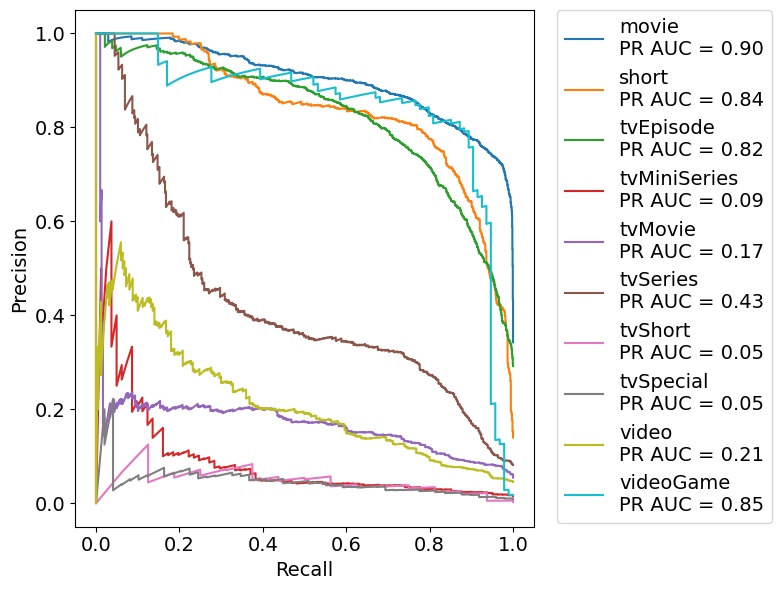
\includegraphics[width=0.9\columnwidth]{../results/images/GaussianNB_PRcurve_tts.png}
    \caption{PR curves (1-vs-rest) for GaussianNB.}
    \label{fig:GaussianNB_PRcurve_tts.png}
\end{figure}

\begin{figure}[ht]
    \centering
    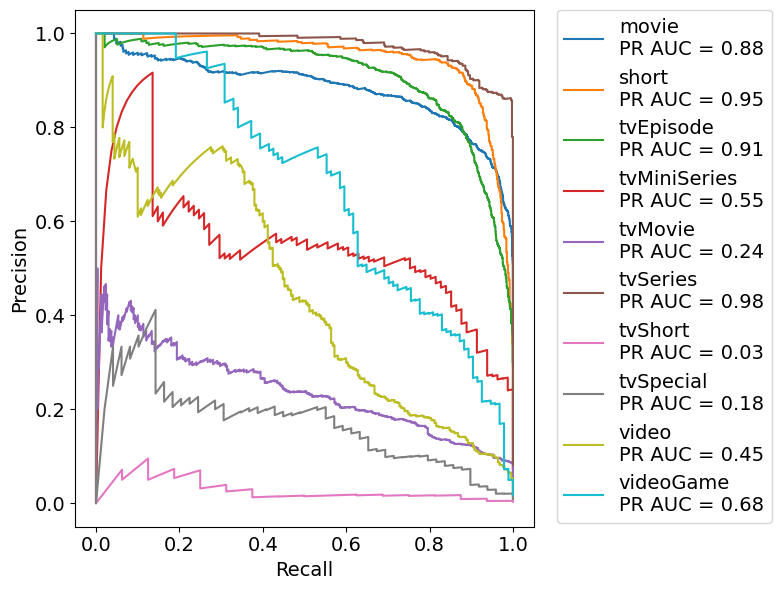
\includegraphics[width=0.9\columnwidth]{../results/images/CatNB_PRcurve_tts.png}
    \caption{PR curves (1-vs-rest) for CategoricalNB.}
    \label{fig:CatNB_PRcurve_tts.png}
\end{figure}

\subsubsection{Target: \textit{binned rating}}
On this task, the performance of the two models was less satisfactory. Nevertheless, both outperformed the baseline, with the CategoricalNB model performing once again better than the GaussianNB model, though less markedly (cf. Table \ref{tab:gnb_cnb_comparison_rating}).

\begin{table}[ht]
    \centering
    \small
    \setlength{\tabcolsep}{4pt}
    \renewcommand{\arraystretch}{0.9}
    \begin{tabular}{l|cccc}
    \hline
    \textbf{Model} & \textbf{Accuracy} & \textbf{Macro F1} & \textbf{ROC AUC} & \textbf{PR AUC} \\
    \hline
    GNB & 0.345 & 0.330 & 0.630 & 0.348 \\
    CNB & 0.427 & 0.387 & 0.680 & 0.398 \\
    \hline
    \end{tabular}
    \caption{Performance of GaussianNB and CategoricalNB models on \textit{binned rating}.}
    \label{tab:gnb_cnb_comparison_rating}
\end{table}
For the GaussianNB model, the confusion matrix (Figure \ref{fig:conf_matr_rating_NB.png}) shows confusion amongst all classes, in particular w.r.t Medium-High, the most popular class (which is the one with the best recall and F1, 0.494 and 0.428): it gets predicted the most. Medium-Low has a particularly low recall (0.173): its records are classified more frequently as any other class (especially as Medium-High and Low) than as itself. 
High and Medium-High are mostly confused among themselves, this is especially true for High, which has the lowest precision (0.251).

The Categorical NB model's overall performance is better than the Gaussian's, but actually this is mostly due to the great improvement of the Low class (F1 went from 0.361 to 0.55): 2/3 of its records are now classified correctly, the misclassified ones are quite balanced among the three remaining classes. All other classes have has a slight decrease in macro F1.
Medium-Low has had a decrease in recall for a slight improvement in precision; less records are classified correctly, but now it is mostly confused with Low.
Medium-High and High both had an improvement in precision, at the cost of recall. The improvement in this model's scoring and ranking capability is better visualized by the PR curves in Figure \ref{fig:PRcurves_rating_NB.png}: the precision for Low and Medium-High is more stable across different thresholds.
\begin{figure}[ht]
    \centering
    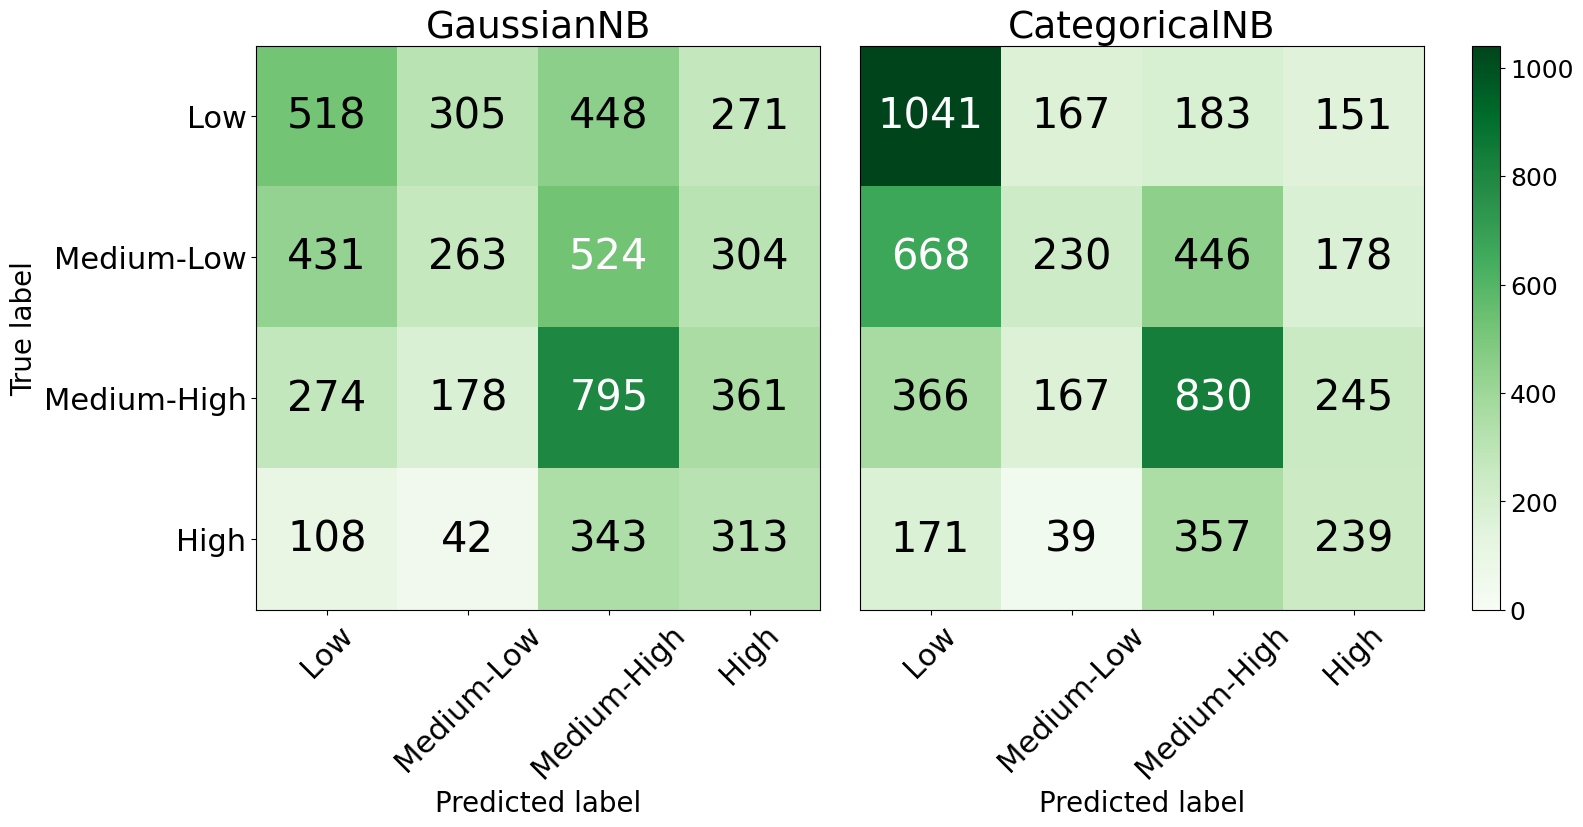
\includegraphics[width=\columnwidth]{../results/images/conf_matr_rating_NB.png}
    \caption{Confusion matrixes for GaussianNB and CategoricalNB for \textit{binned rating}.}
    \label{fig:conf_matr_rating_NB.png}
\end{figure}
\begin{figure}[ht]
    \centering
    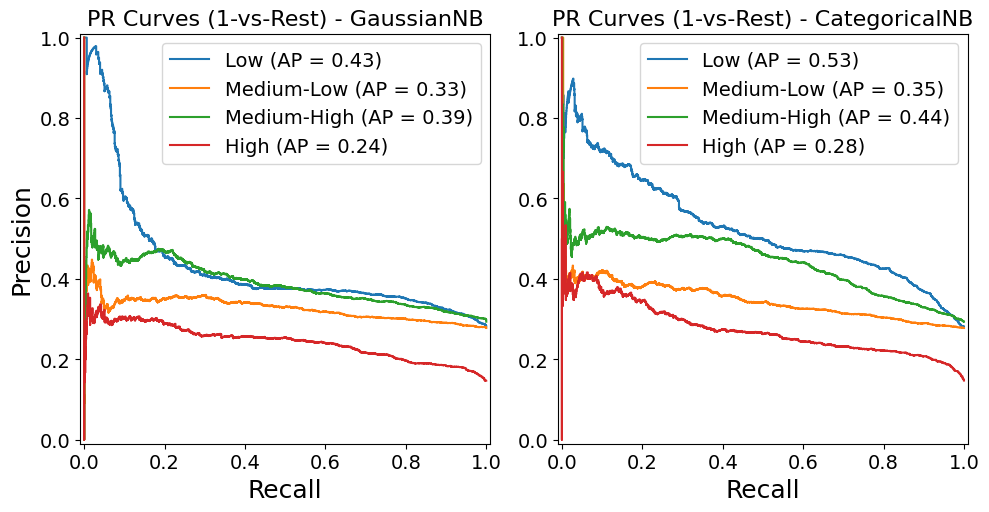
\includegraphics[width=\columnwidth]{../results/images/PRcurves_rating_NB.png}
    \caption{PR curves for GaussianNB and CategoricalNB for \textit{binned rating}.}
    \label{fig:PRcurves_rating_NB.png}
\end{figure}

\subsection{Decision Tree Classifier}
\label{naive_bayes}
\subsubsection{Target: \textit{titleType}}
\subsubsection{Target: \textit{binned rating}}